\documentclass[10pt,a4paper]{article}
\newcommand{\runningtitle}{Neural topic scores in diabetic foot ulcer research}
\usepackage[margin=15mm,top=16mm,bottom=17mm,headheight=12pt,headsep=5mm,footskip=9mm]{geometry}
\usepackage{fontspec}
\setmainfont{TeX Gyre Termes}
\setsansfont{Arial}
\usepackage{amsmath,amssymb,mathtools,bm}
\usepackage{unicode-math}
\setmathfont{TeX Gyre Termes Math}
\usepackage{graphicx,booktabs,array,tabularx,longtable}
% Keep captions visually separated from their artwork/table rules, while
% retaining a compact single-column manuscript.  The same defaults are used
% by both papers so appendix tables and main-text figures do not drift apart.
\usepackage[font=small,labelfont=normalfont,labelsep=period,skip=8pt]{caption}
\usepackage{flafter,placeins,needspace}
\usepackage[sort&compress,numbers]{natbib}
\usepackage[unicode,colorlinks=true,linkcolor=black,citecolor=black,urlcolor=black]{hyperref}
% longtable 4.24 uses infinitely shrinkable glue before a kernel box split.
% Backport the upstream 4.25 finite-shrink fix (latex3/latex2e issue 1907)
% locally. etoolbox is already loaded by hyperref; no runtime/package changes.
% Patch both nested vbox branches. Already-fixed versions are left unchanged.
\makeatletter
\patchcmd{\LT@output}{\vss}{\vskip\z@\@plus1fil\@minus\normalbaselineskip}{}{}
\patchcmd{\LT@output}{\vss}{\vskip\z@\@plus1fil\@minus\normalbaselineskip}{}{}
\makeatother
\usepackage{xcolor,microtype,titlesec,enumitem,fancyhdr}
\usepackage{bookmark}
\hypersetup{pdfcreator={XeLaTeX},pdfauthor={Zeyu Fu}}
\graphicspath{{figures/}}
\setlength{\parindent}{1em}
\setlength{\parskip}{1pt plus .4pt}
\linespread{1.02}
\setlength{\textfloatsep}{12pt plus 2pt minus 1pt}
\setlength{\floatsep}{10pt plus 2pt minus 1pt}
\setlength{\intextsep}{12pt plus 2pt minus 1pt}
\renewcommand{\topfraction}{.94}
\renewcommand{\bottomfraction}{.88}
\renewcommand{\textfraction}{.06}
\renewcommand{\floatpagefraction}{.78}
\setcounter{topnumber}{3}
\setcounter{bottomnumber}{2}
\setcounter{totalnumber}{4}
\setlength{\abovedisplayskip}{4pt plus 1pt minus 2pt}
\setlength{\belowdisplayskip}{4pt plus 1pt minus 2pt}
\setlength{\abovedisplayshortskip}{2pt plus 1pt}
\setlength{\belowdisplayshortskip}{3pt plus 1pt}
\titlespacing*{\section}{0pt}{8pt plus 1pt minus 2pt}{3pt}
\titlespacing*{\subsection}{0pt}{6pt plus 1pt minus 1pt}{2pt}
\titleformat{\section}{\large\bfseries}{\thesection}{.6em}{}
\titleformat{\subsection}{\normalsize\bfseries}{\thesubsection}{.6em}{}
\setlist{nosep,leftmargin=1.7em,topsep=4pt}
\setlength{\bibsep}{1.5pt}
\renewcommand{\bibfont}{\small\let\emph\textnormal}
\setlength{\tabcolsep}{4pt}
% Longtable captions sit above the first rule.  These pre/post skips prevent
% adjacent appendix tables from reading as one continuous table while still
% allowing a continued table head to remain visually attached to its rows.
\setlength{\LTpre}{8pt plus 2pt minus 1pt}
\setlength{\LTpost}{8pt plus 2pt minus 1pt}
\setlength{\LTcapwidth}{\textwidth}
\captionsetup[figure]{skip=8pt}
\captionsetup[table]{skip=8pt}
\captionsetup[longtable]{font=footnotesize,skip=8pt}
\renewcommand{\arraystretch}{1.12}
\setlength{\emergencystretch}{1.2em}
\widowpenalty=10000
\clubpenalty=10000
\raggedbottom
\pagestyle{fancy}
\fancyhf{}
\fancyhead[L]{\sffamily\fontsize{8}{10}\selectfont\runningtitle}
\fancyfoot[C]{\small\thepage}
\renewcommand{\headrulewidth}{.25pt}
\newcommand{\papertitle}[1]{\thispagestyle{plain}\begin{center}\vspace*{-5mm}{\fontsize{19}{22}\selectfont\bfseries #1\par}\vspace{2mm}{\normalsize Zeyu Fu\par}\end{center}\vspace{-2mm}}
\newcommand{\paperfigure}[3]{\begin{figure}[!htbp]\centering\includegraphics[width=\linewidth]{#1.pdf}\caption{#3}\label{#2}\end{figure}}
\newcommand{\supplement}{\FloatBarrier\section*{Supplementary methods and numerical results}\addcontentsline{toc}{section}{Supplementary methods and numerical results}\setcounter{section}{0}\setcounter{table}{0}\setcounter{equation}{0}\renewcommand{\thesection}{S\arabic{section}}\renewcommand{\thetable}{S\arabic{table}}\renewcommand{\theequation}{S\arabic{equation}}\renewcommand{\theHsection}{supp.\arabic{section}}\renewcommand{\theHtable}{supp.\arabic{table}}\renewcommand{\theHequation}{supp.\arabic{equation}}}
\newcolumntype{L}{>{\raggedright\arraybackslash}X}
\newcommand{\doi}[1]{\href{https://doi.org/#1}{doi: #1}}
\newcommand{\E}{\mathbb{E}}
\newcommand{\R}{\mathbb{R}}
\newcommand{\ind}{\mathbf{1}}

\hypersetup{pdftitle={Neural topic modelling of fibroblast measurements and diabetic foot ulcer healing: a patient-level audit}}

\title{Neural topic modelling of fibroblast measurements and diabetic foot ulcer healing: a patient-level audit}
\author{Zeyu Fu$^{1,*}$\\[3pt]\small $^1$State Key Laboratory of Trauma and Chemical Poisoning,\\\small Institute of Combined Injury, Chongqing Engineering Research Center for Nanomedicine,\\\small College of Preventive Medicine, Army Medical University, Chongqing, China\\\small $^*$Correspondence: \texttt{fuzeyu09@gmail.com}; \texttt{fuzeyu99@126.com}}\date{}
\vfuzz=1pt
\usepackage{float}
\usepackage[switch]{lineno}
\begin{document}
\maketitle
\modulolinenumbers[5]\linenumbers
\begin{abstract}
A cell population can have a high average programme score because more cells have high scores, even when expression within those cells changes little. We examined this distinction for a fibroblast-associated neural topic measurement in diabetic foot ulcers. The primary healing comparison used 11 patients. We separated the average score into cell prevalence and within-group contributions, checked technical sensitivity, and repeated topic selection within the evaluation. Cell prevalence dominated the average, but the two summaries share the same measurements and their agreement is not independent evidence for a distinct biological state. High-scoring cells also occurred in intact skin. Patient-level healing contrasts remained uncertain, and accounting for selection of the topic did not establish a healing association. Models that selected the topic using the training patients did not establish predictive performance. The measurement therefore describes the composition of sampled fibroblasts without demonstrating a unique cell state or a clinically useful healing predictor. Amputation was not measured, and independent outcome validation remains necessary.
\end{abstract}
\noindent\textbf{Keywords:} topic models; construct validity; fibroblasts; wound healing; CHI3L1; patient-level inference.

\section{Introduction}
Diabetic foot ulcers develop in tissue where neuropathy, vascular impairment, inflammation and repeated injury can coexist. Closure does not remove the risk of recurrence, making it important to understand which tissue measurements describe the current wound and which might inform its subsequent course \citep{armstrong2017,wilkinson2020}. Single-cell profiling has identified fibroblast-associated programmes that differ between healing groups in diabetic-foot skin \citep{theocharidis2022,geo_gse165816}. These observations motivate prognostic research, but a programme score first needs a defensible measurement interpretation. An average expression loading can change for several reasons, and those reasons imply different biological experiments and different validation requirements.

Fibroblasts are particularly relevant to this problem because their transcriptional diversity reflects both tissue organization and responses to injury. Experimental lineage studies in mouse skin distinguish fibroblast populations with different contributions to dermal architecture and repair \citep{driskell2013}. Single-cell comparisons across organs identify substantial variation in extracellular-matrix programmes and distinguish fibroblasts from related mural populations \citep{muhl2020}. A broader atlas describes shared and specialized fibroblast states across tissues and disease contexts \citep{buechler2021}. These findings support careful study of fibroblast heterogeneity; they do not imply that a gene programme observed in one wound cohort corresponds to a universal cell type or carries the same clinical meaning in another.

The tissue context also matters within a nominally common cell class. Human skin profiling has associated aging with changes in fibroblast transcriptional organization \citep{soleboldo2020}. Anatomical site, the depth and location of a biopsy, and the cells recovered during processing can therefore be relevant to the interpretation of a tissue summary \citep{philippeos2018}. A score enriched for matrix and inflammatory genes may capture a reproducible aspect of that context without being specific to successful repair. The central question is whether differences in its mean primarily describe how strongly cells express the programme, how many high-scoring cells are recovered, or a combination of these contributions.

Topic models and gene-expression decompositions provide ways to represent such heterogeneity without requiring every cell to belong to one expression programme \citep{blei2003,kotliar2019}. Neural latent-variable models offer another means of summarizing high-dimensional expression for subsequent comparisons \citep{lopez2018}. Autoencoding topic inference and Gaussian reparameterization supply the computational background for the neural representation used here \citep{srivastava2017,kingma2014}. This implementation uses a logistic-normal coordinate and a regularized reconstruction loss on cell proportions, rather than a Dirichlet prior or a fitted negative-binomial count model. Fitted coordinates acquire meaning through that objective, the gene panel, normalization and sampling scheme. A simplex constraint makes the coordinates compositional; it does not independently calibrate a coordinate as the probability of a biological state \citep{aitchison1980}. Changes in cell composition and changes within a compartment must consequently be distinguished when interpreting a biopsy-level average \citep{buettner2021}.

Defining a high state by a threshold makes one aspect of the measurement easy to communicate, but it also discards variation within the two resulting bins. The general information loss from dichotomizing continuous measurements is well established \citep{altman2006}. In single-cell analysis, neighborhood-based abundance methods provide an alternative to treating every cluster boundary as biologically fixed \citep{dann2022}. Neither approach removes the need to specify the denominator and independent sampling unit. A correlation between a mean and a threshold fraction is especially difficult to interpret mechanistically because both summaries are calculated from the same cell scores. An explicit decomposition of the mean can expose the terms that a simple abundance interpretation treats as approximately constant \citep{buettner2021}.

Technical effects can modify both the score and the cells assigned to a compartment. Tissue dissociation can induce expression programmes, extracellular RNA can enter measured profiles, and doublets can combine transcripts from different cell types \citep{vandenbrink2017,young2020,wolock2019}. Quality control, depth matching and exclusion rules address particular parts of this problem, with consequences that depend on the retained population \citep{heumos2023}. Normalized expression proportions also differ from residual-based variance stabilization, so normalization methods should not be treated as interchangeable measurements \citep{hafemeister2019}. Across studies, a common representation also has to balance preservation of biological variation against technical alignment \citep{luecken2022}. Technical robustness therefore supplies evidence about the stability of a measurement under specified perturbations, while leaving its disease specificity and prognostic value to be evaluated separately.

Clinical inference imposes a further distinction between cells, specimens and patients. Repeated biopsies can characterize tissue heterogeneity, but they do not create independent healing outcomes. Methods for multi-sample expression and abundance comparisons preserve this dependence rather than treating every recovered cell as a replicate \citep{crowell2020,squair2021,zimmerman2021,lazic2010}. Outcome discrimination is only one aspect of a clinically useful predictor: agreement between predicted and observed risks and the consequences of decisions at relevant thresholds also matter \citep{steyerberg2010,vancalster2019,vickers2006}. Reporting and validation should match that intended use \citep{collins2015}. In a small discovery cohort, selecting among readouts can produce optimistic performance estimates, and a nonsignificant contrast does not establish equivalence \citep{cawley2010,schuirmann1987,lakens2017}. Requirements for prediction-model development depend on outcome frequency, model complexity and anticipated performance rather than a universal sample-count rule \citep{riley2019}.

The biological material should remain visible throughout this measurement argument. A dissociated-cell atlas describes the populations that survived sampling and processing, while gene-level summaries show the expression context from which a programme was inferred. Neither is a spatial reconstruction of the wound. Similarly, coloring an embedding by a score is a way to inspect its distribution, not an independent test of the score's biological validity. Embedding algorithms can alter apparent separation and density, making their connection to the input measurements and the inferential unit essential to interpretation \citep{becht2019,huang2022visualization}.

We examine a frozen fibroblast-associated topic in public diabetic-foot skin data as a tissue measurement and an exploratory healing readout \citep{theocharidis2022,cronbach1955}. Amputation risk is the clinical context, not a measured endpoint of this audit; a healing-category comparison is not an estimate of amputation risk. The analysis distinguishes mean loading within fibroblasts, the fraction above a fitted threshold and the mean over all recovered cells. Distributional decomposition and technical perturbations examine what these readouts measure. Author-mapped patient comparisons and paired anatomical controls examine which contrasts they can support, while external wound datasets extend the tissue contexts in which the frozen score can be evaluated. This design connects measurement interpretation to clinical inference without assuming that evidence for one is sufficient for the other \citep{collins2015}.

\section{Results}
\subsection{The average score mainly reflects the prevalence of high-scoring cells}
The primary question was whether a fibroblast-associated topic measurement established a healing association beyond its relationship with cell prevalence. The discovery data comprised 25 specimens from 20 patients, with healing comparisons restricted to seven healed and four non-healed ulcer patients. The workflow distinguishes fibroblast mean score, above-cut fraction and all-cell patient summaries (Figure~\ref{fig:p1f1}a). The lineage and loading displays use the same observed cells, while marker expression, the fibroblast score distribution and specimen composition describe their context (Figure~\ref{fig:p1f1}b--f). These measurements do not establish a new biological cell identity.

\begin{figure}[H]\centering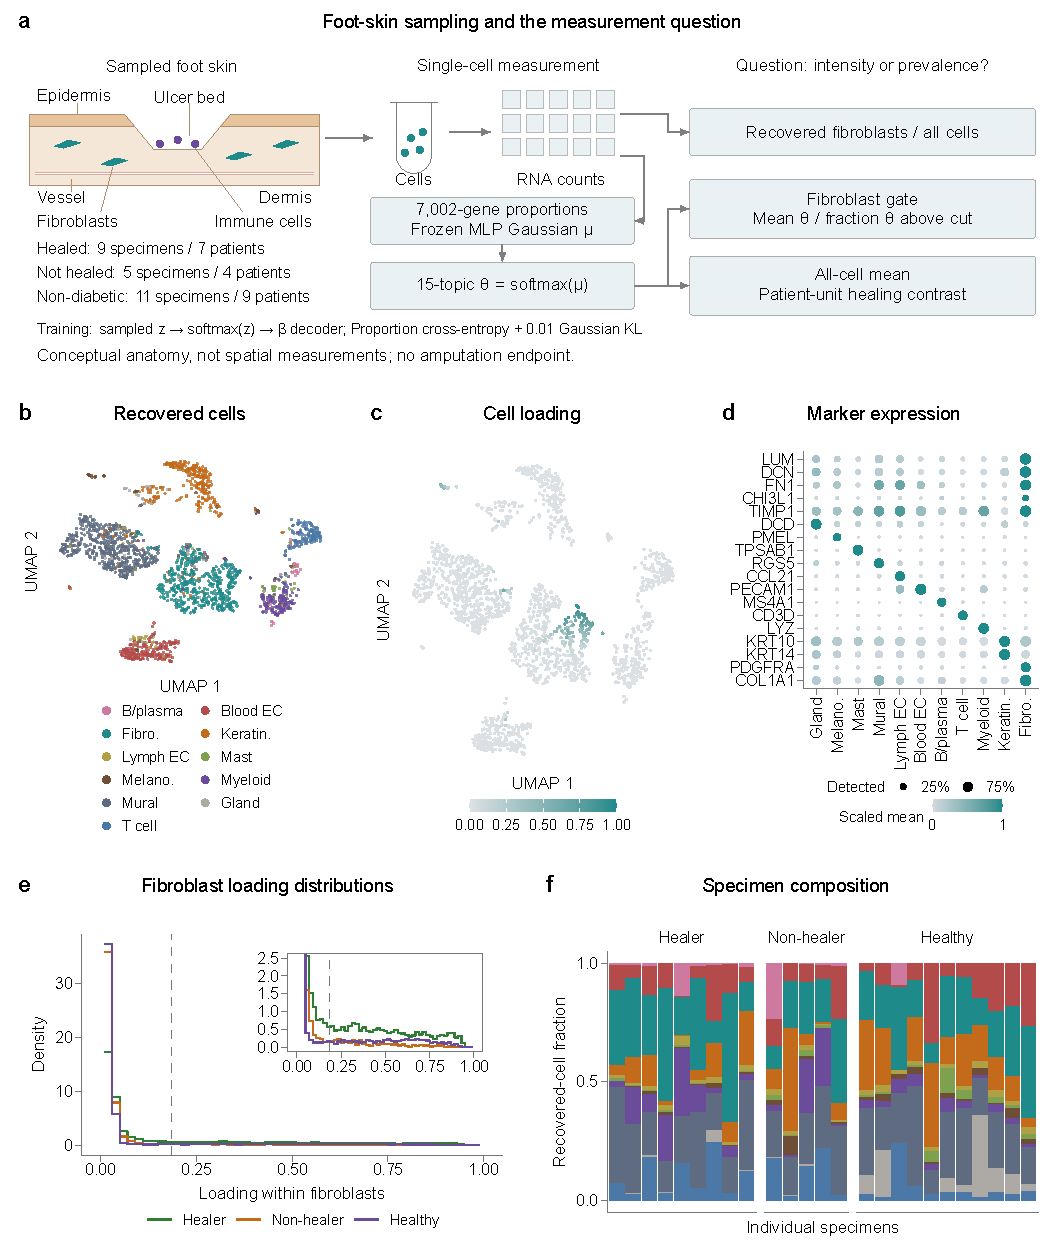
\includegraphics[width=\linewidth]{journal-figures/paper1_figure1_workflow.pdf}
\caption{What is measured in diabetic-foot skin? (a) Conceptual foot skin and destructive sampling, not measured histology. The 25 specimens represent 7 healed, 4 non-healed and 9 non-diabetic people. Composition uses recovered-cell counts; frozen inference maps 7,002-gene proportions through Gaussian mean μ to 15-topic softmax θ. Fibroblast mean/fraction and the all-cell patient mean are separate summaries. Neither readout feeds the other. Training: sampled z, normalized decoder β, cross-entropy plus 0.01 Gaussian KL. No amputation endpoint is measured. (b) Uniform display of 2,000 of 76,461 cells by marker-derived lineage; Fibro., fibroblast; EC, endothelial; mural, pericyte/smooth muscle. (c) The same cells by loading. (d) Expression: size is detection fraction, color gene-wise scaled mean log-normalized expression. Annotation markers are not independent label validation. (e) All 19,410 fibroblast loadings with the original cut; inset expands density 0--2.5, preserving the spike. (f) Composition in 25 specimens; colors match b. Non-diabetic people lack healing outcomes; inference uses full data and patient units.}\label{fig:p1f1}\end{figure}
\FloatBarrier

The mean and high-score fraction were strongly associated: specimen Spearman correlation was 0.933, and pooling repeated specimens gave a patient correlation of 0.937 (Figure~\ref{fig:p1f2}a--c). Score distributions and within-bin averages nevertheless varied (Figure~\ref{fig:p1f2}d--f). Both summaries use the same cells, so their correlation cannot independently validate two biological states. The exact decomposition provides the more limited interpretation that the mean is largely a population-composition readout.

\begin{figure}[H]\centering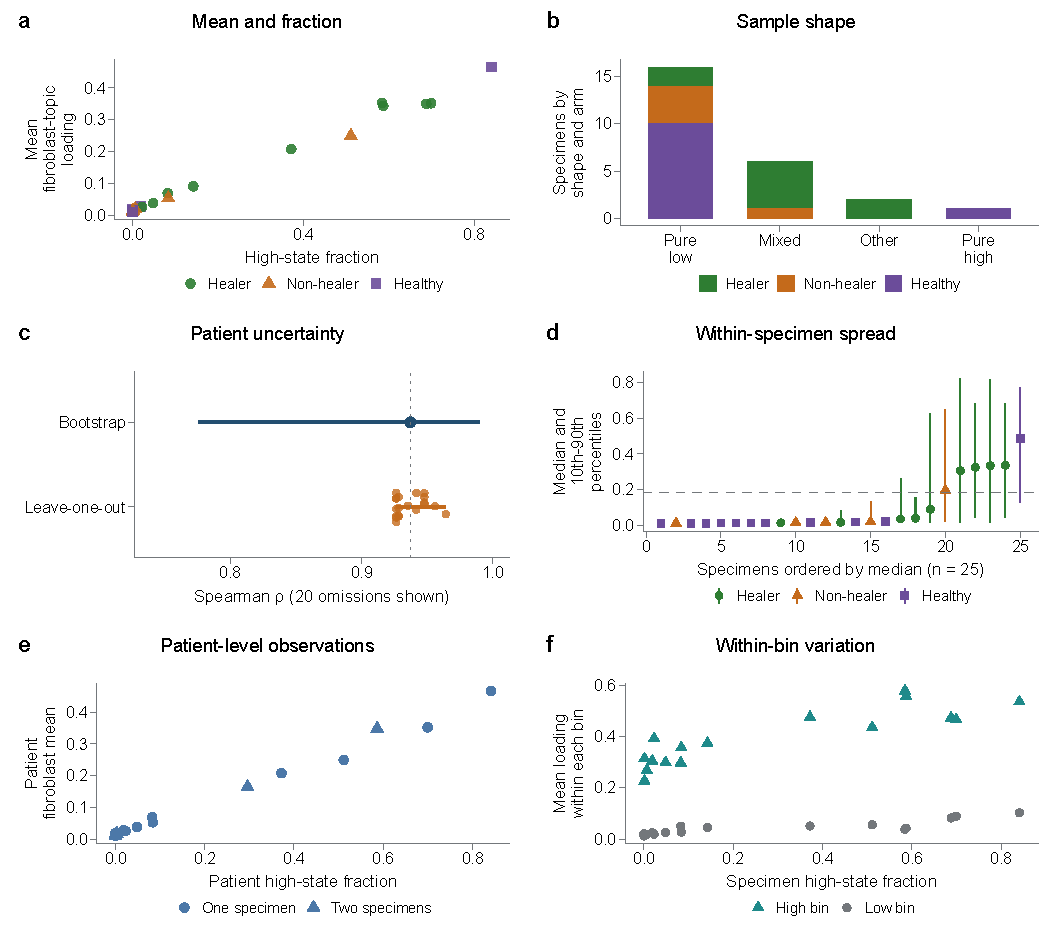
\includegraphics[width=\linewidth]{journal-figures/paper1_figure2_mixture_semantics.pdf}
\caption{Mean, prevalence and within-bin variation. (a) The 25 specimens comprise 9 healing, 5 non-healing and 11 non-diabetic samples; the cut is 0.1842958 and Spearman ρ=0.933. (b) Stacks retain clinical-arm composition in quantile-defined shapes: pure low has the 90th percentile at most 0.15, pure high the 10th percentile at least 0.10, and mixed the 10th percentile at most 0.05 and 90th percentile at least 0.40. (c) After fibroblast-count pooling to 20 patients, ρ=0.937; blue is the saved patient-bootstrap 95\% interval, while orange shows all 20 omission estimates and their range. Vertical jitter separates identical correlations. (d) Ordered specimen medians and 10th--90th percentiles are loading distributions, not confidence intervals. (e) All 20 patient means and fractions; symbols identify one or two contributing specimens, not outcome groups. (f) Low- and high-bin means against specimen high fraction; undefined empty-bin means are not plotted. These shared-cell summaries do not identify discrete biological states, constant component intensities or a healing effect.}\label{fig:p1f2}\end{figure}
\FloatBarrier

\subsection{Technical stability is conditional on the measurement pipeline}
Selected stress, panel-depth and immune-transcript controls retained aspects of the original pattern (Figure~\ref{fig:p1f3}a--c). The depth-matching agreement conditions on the original lineage labels. Immune-covariate and placebo residual comparisons both favored one component, so the fitted two-component description was not invariant to those transformations. Full count thinning and repeated quality filtering changed cell retention and lineage assignment (Figure~\ref{fig:p1f3}d,e). Patient contrasts retained computational sensitivity across the thinning seeds (Figure~\ref{fig:p1f3}f). The controls support a bounded description of the frozen measurement; they do not establish whole-pipeline invariance or clinical portability.

\begin{figure}[H]\centering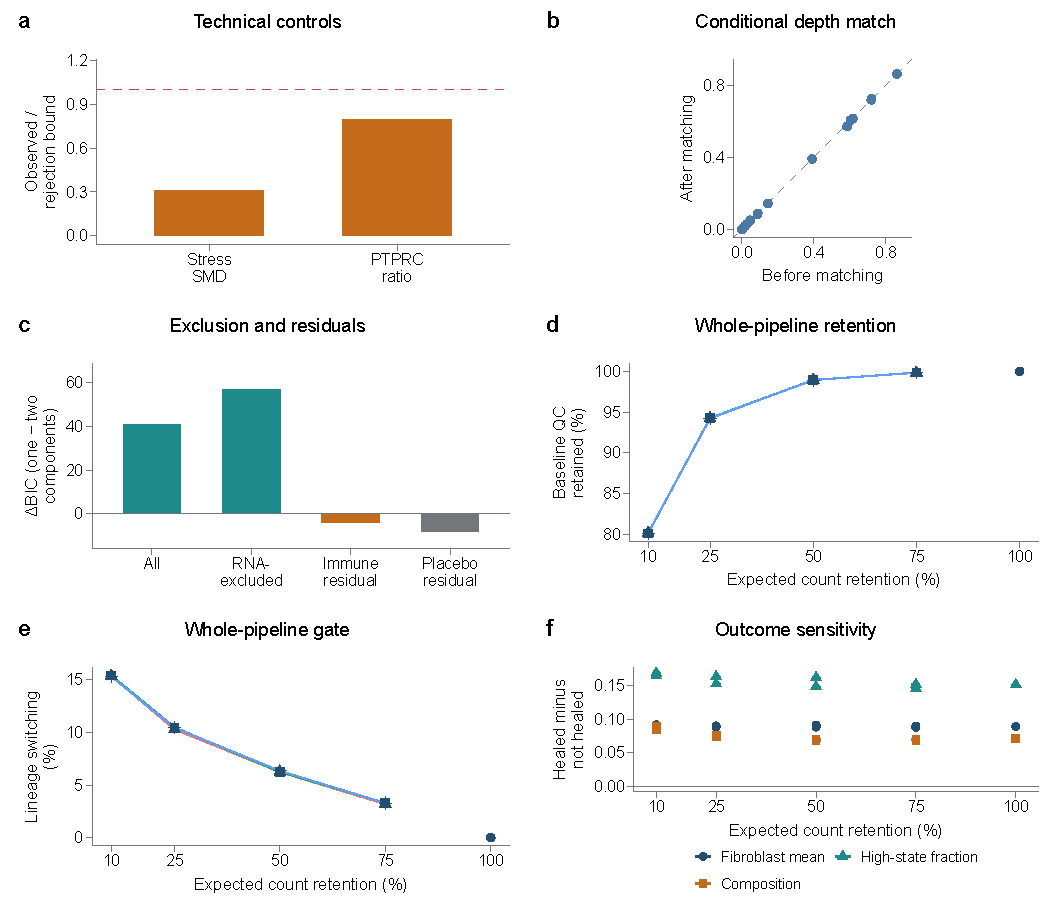
\includegraphics[width=\linewidth]{journal-figures/paper1_figure3_artifact_controls.pdf}
\caption{Conditional controls and whole-pipeline sensitivity. (a) Stress SMD and PTPRC rate ratio divided by their rejection bounds; dashed line: one. (b) Specimen fractions before and after matching 14,561 eligible fibroblasts to 986 panel counts; identity is dashed. The 99.5\% agreement conditions on original lineage labels. (c) One-minus-two-component BIC for 24 matched specimens before and after immune-transcript exclusion, and separately for immune- and placebo-covariate residuals in 25 specimens. Both residual comparisons favor one component; their samples and perturbations are not interchangeable. (d) Retention of baseline QC survivors after count thinning and rerunning QC. (e) Lineage switches among common survivors. d/e retain all three computational seeds and the unthinned baseline. (f) Seed minima and maxima of patient contrasts for three readouts; these ranges are sensitivities, not confidence intervals. The same 7 healed and 4 non-healed patients, frozen gate, encoder and cut are used. Conditional stability does not establish whole-pipeline invariance, identity truth or clinical portability.}\label{fig:p1f3}\end{figure}
\FloatBarrier

\subsection{Patient-level healing contrasts remain uncertain}
The healed-minus-non-healed contrasts were 0.0892 for fibroblast mean score, 0.1514 for above-cut fraction and 0.0708 for fibroblast composition. Exhaustive probabilities over all 330 label allocations were 0.3121, 0.3697 and 0.4697, respectively, with a common Benjamini--Hochberg adjusted value of 0.4697 (Figure~\ref{fig:p1f5}a--c). All patient-bootstrap intervals included zero. This uncertainty permits neither a validated healing signal nor equivalence of the outcome groups.

\begin{figure}[H]\centering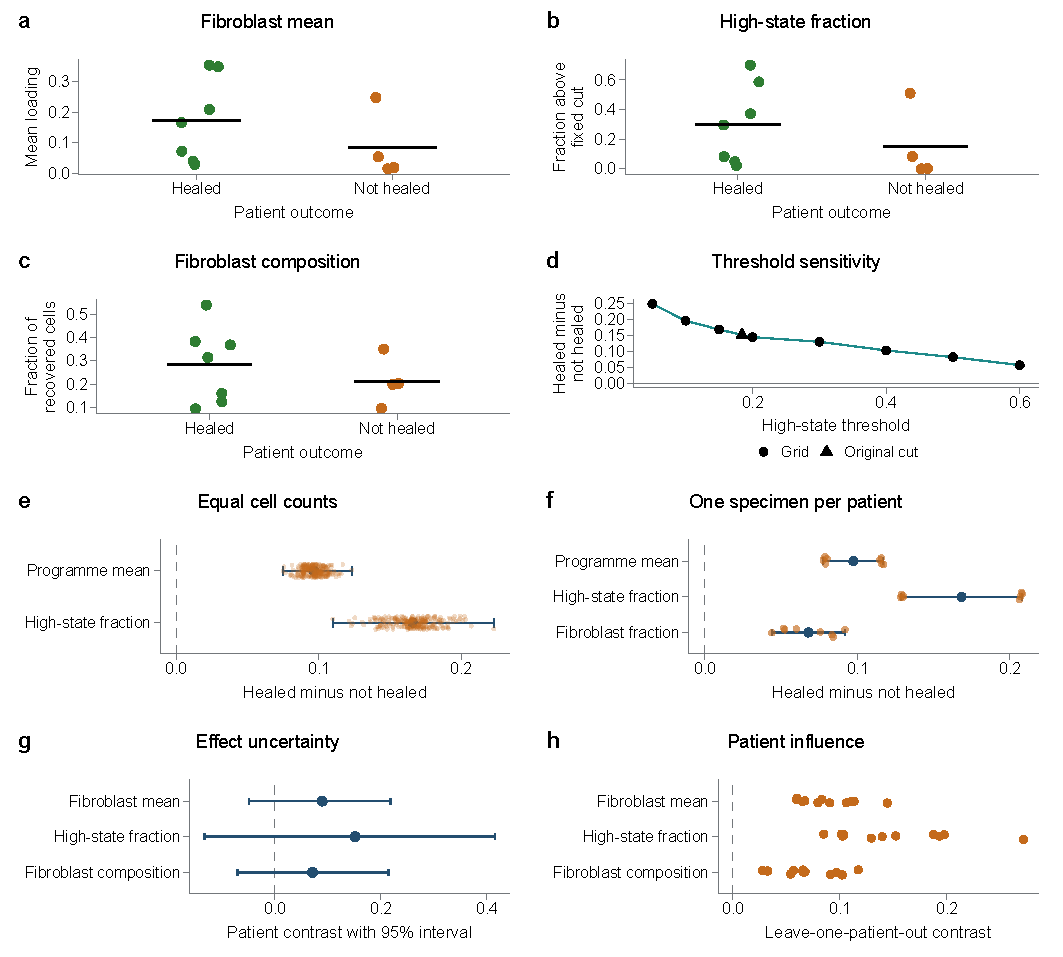
\includegraphics[width=\linewidth]{journal-figures/paper1_figure5_patient_readouts.pdf}
\caption{Patient-unit readouts, uncertainty and influence. a--c show 7 healed and 4 non-healed DFU patients, with group means; repeated specimens are pooled using the relevant cell counts. (a) Mean fibroblast loading: difference 0.0892, exact p=0.3121. (b) Fraction above the frozen cut: difference 0.1514, p=0.3697. (c) Fibroblast fraction: difference 0.0708, p=0.4697. Tests use all 330 label allocations; BH q=0.4697 for all three. (d) High-state contrasts across eight fixed cuts and the original midpoint. (e) All 250 saved equal-cell draw contrasts, their means and full ranges, using 100 fibroblasts per specimen. (f) All eight one-specimen-per-patient choices, with means and full ranges. Vertical jitter separates saved values without changing their contrasts. (g) Cell-count-weighted effects with 10,000-draw patient-bootstrap 95\% intervals; all span zero. (h) All 11 patient omissions per readout. e, f and h describe the same patients, not confidence intervals or independent replications; positive omission estimates and intervals spanning zero can coexist without validating prognosis or equivalence.}\label{fig:p1f5}\end{figure}
\FloatBarrier

Threshold variation, equal-cell draws and one-specimen-per-patient choices characterize sensitivity in the same 11 patients (Figure~\ref{fig:p1f5}d--f). Cell-count-weighted intervals and leave-one-patient-out estimates describe different aspects of those observations (Figure~\ref{fig:p1f5}g,h). Computational repeats and positive omission estimates do not add outcomes or turn an uncertain interval into evidence for prognosis.

\subsection{Held-pair discrimination and anatomy do not provide outcome validation}
Patient-pair comparisons fit on the other nine patients and preserve all 28 held pairs. Their wins, ties and losses are dependent because the same seven healed and four non-healed patients recur (Figure~\ref{fig:p1f8}a). Topic-selection checks confined to the training patients did not establish predictive performance beyond the discovery-trained representation.

\begin{figure}[H]\centering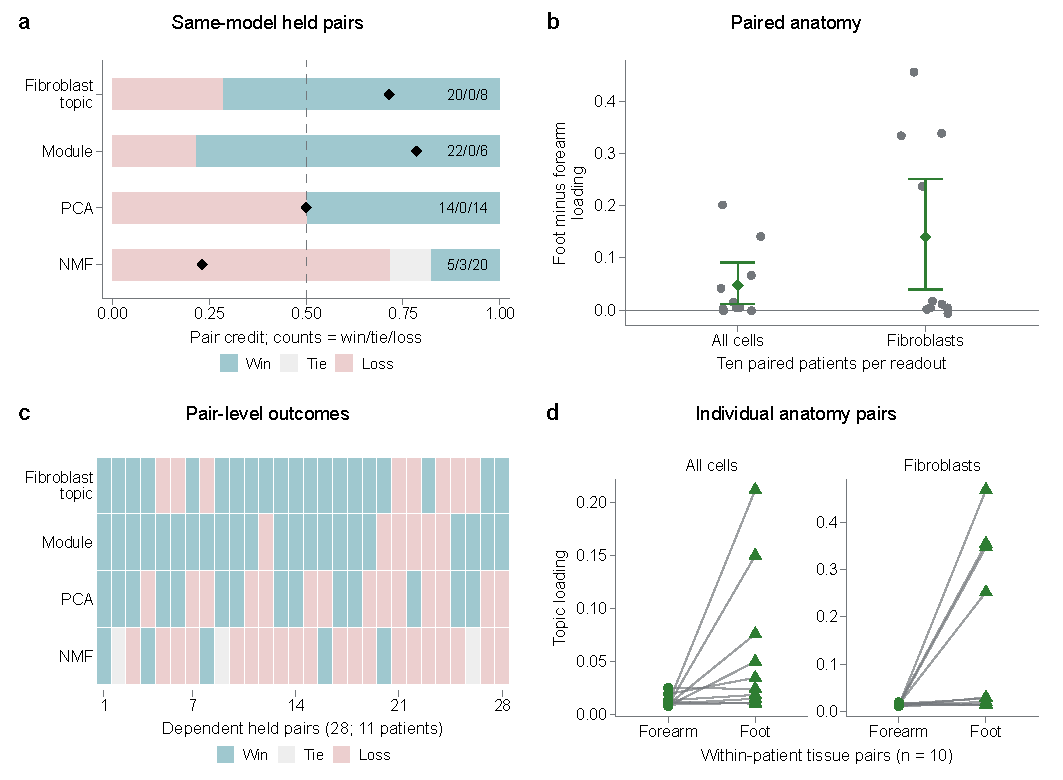
\includegraphics[width=\linewidth]{journal-figures/paper1_figure8_patient_unit_anatomy.pdf}
\caption{Patient-pair discrimination and anatomical sensitivity. (a) Win/tie/loss fractions and counts for each scoring method, with a black diamond at its mean credit across 28 held pairs. Every fold fits on the other nine patients; ties earn half credit. The pairs share 7 healed and 4 non-healed patients and have no binomial confidence interval. (b) All 10 paired foot-minus-forearm differences for both all-cell and fibroblast-restricted loading, overlaid with saved means and paired-patient bootstrap 95\% intervals. For the all-cell topic, sign-flip p=0.0107 and BH q=0.0402. (c) All dependent held-pair wins, ties and losses in saved order. (d) The same 10 patients' forearm and foot levels, separately for the two cell denominators with distinct vertical scales. b and d are different summaries of the same pairs, not 20 independent people. Neither this anatomical sensitivity nor the shared-patient scoring comparison supplies independent clinical validation.}\label{fig:p1f8}\end{figure}
\FloatBarrier

Paired foot--forearm comparisons retain ten patients and show sensitivity to anatomical site and cell denominator (Figure~\ref{fig:p1f8}b). The foot specimens mix ulcers with intact skin. Every held-pair win, tie and loss is retained (Figure~\ref{fig:p1f8}c); the same ten paired patients' site-specific levels provide the complementary anatomical view (Figure~\ref{fig:p1f8}d). These pairs therefore assess tissue context rather than independent healing specificity. The external projections and detailed pairwise comparisons are given in the Supplementary Information.

\subsection{Topic selection and intact skin limit the biological interpretation}
Topic 0 was named after its clinical-arm means were inspected. Its observed all-cell healed/non-healed ratio of 1.96 was below the median largest ratio of 2.28 under random labels. Repeating selection over all topics gave adjusted probabilities of 0.785 for the all-cell readout, 0.609 for fibroblast mean score and 0.955 for the fit-specific above-cut fraction (Figure~\ref{fig:p1f11}a). The selected topic therefore did not establish a healing association after accounting for that selection.

\begin{figure}[H]\centering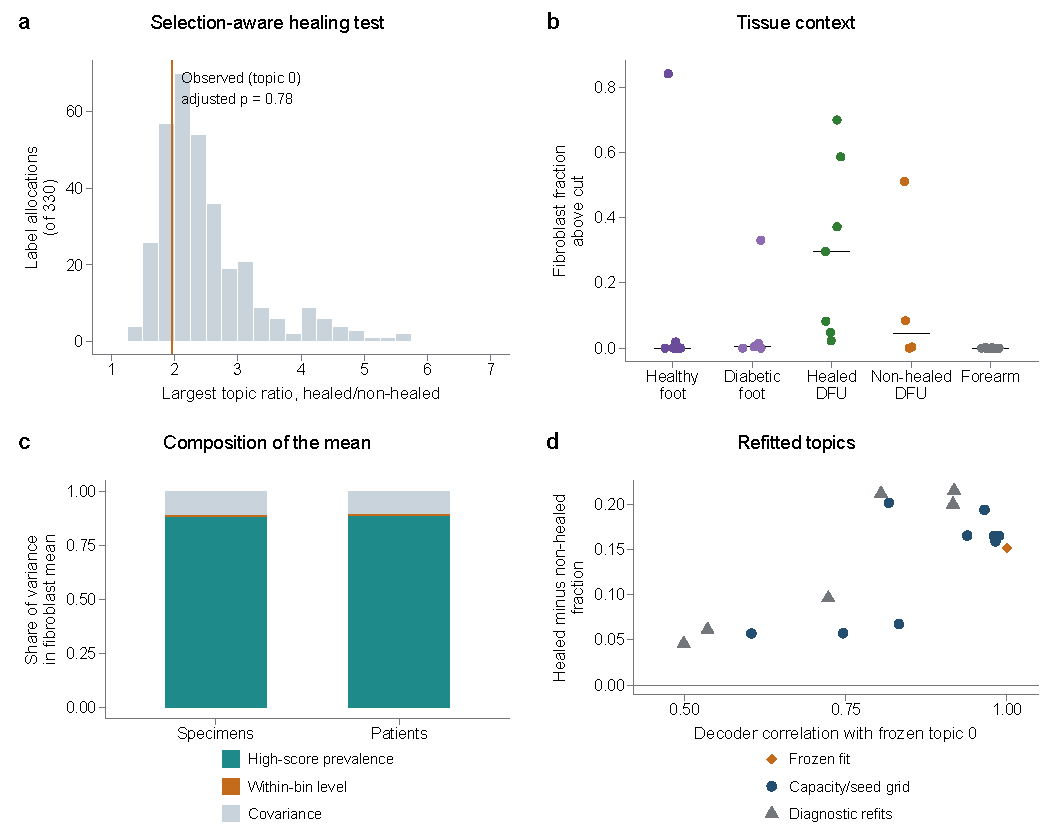
\includegraphics[width=\linewidth]{journal-figures/paper1_figure11_selection_context.pdf}
\caption{Selection, tissue context and composition of the fibroblast readout. (a) Each of the 330 allocations of 7 healed among the 11 DFU patients gives the largest healed/non-healed all-cell mean ratio over the 15 topics; the orange line is the observed ratio of topic 0, which was named after its arm-wise means were inspected, and the adjusted p is the fraction of allocations at least as extreme. (b) Patient-level fraction of fibroblasts above the frozen cut in intact healthy and diabetic foot skin, healed and non-healed ulcers, and forearm skin from all groups; bars are medians. (c) Shares of between-unit variance in the fibroblast mean from the high-score prevalence term, the within-bin level term and their covariance in the exact mean decomposition. (d) Healed minus non-healed fraction of fibroblasts above the topic cut for the frozen fit and 15 refits, each scored with its own matched topic and cut, against the decoder correlation of that topic with frozen topic 0; no refit gives an exact permutation p below 0.05.}\label{fig:p1f11}\end{figure}
\FloatBarrier

High-scoring fibroblasts occurred in nine of the 11 ulcer patients and two of 15 intact foot-skin donors (Figure~\ref{fig:p1f11}b). Prevalence accounted for 88\% of the between-specimen variance in the mean and 89\% between patients, alongside within-bin and covariance contributions (Figure~\ref{fig:p1f11}c). Fifteen capacity and initialization refits retained the contrast direction but none reached an exact probability below 0.05 (Figure~\ref{fig:p1f11}d). Taken together, these findings describe a prevalence-dominated measurement without identifying a unique fibroblast programme or demonstrating clinically useful healing prediction.

The supplementary material retains the complete technical controls, patient crosswalk, uncertainty calculations, external projections, anatomical contrasts and design sensitivities. These additional calculations characterize the same observed datasets; no independent outcome-validation cohort or amputation endpoint was available.























\section{Discussion}

The frozen fibroblast readout is enriched in the sampled ulcers, and its mean is dominated by high-score prevalence under the chosen cut. The prevalence term contributed close to nine-tenths of between-specimen and between-patient variance, while within-bin levels and their covariance also contributed.

The nine-fit capacity and initialization audit sharpens the distinction between a measurement association and a reproducible programme identity. Mean--fraction correlations remained high while decoder matches, loading cuts and some person-specific readouts varied substantially.

The patient-unit extension connects the fibroblast interpretation directly to the available healing categories. Averaging programme scores within fibroblasts, counting high-scoring fibroblasts and counting fibroblasts among all cells all gave higher point estimates in healed patients, but each comparison retained considerable uncertainty.

The different uncertainty summaries answer different questions. Patient bootstrap intervals resample the observed outcome arms and inherit the limitations of their small empirical distributions \citep{efron1993}.

The cell atlas and expression profiles also clarify what is still missing experimentally. Melanocytes carried the highest loading, so the score is not a count of one anatomically defined fibroblast population, and doublet removal left the contrasts unchanged.

This distinction has biological consequences. A high mean could accompany recruitment or recovery of a particular fibroblast population, increased expression within an existing population, or changes in several populations at once.

The threshold should be understood as an operational convention. It permits a reproducible high-state fraction and makes the denominator explicit, while assigning nearby scores on opposite sides of the cut to different bins.

The technical controls provide evidence about selected perturbations of this operational measurement. Most state labels survived count matching under fixed lineage assignments, and specimen fractions were stable after specified immune-transcript exclusions.

The difference between a tissue measurement and a healing predictor becomes clearer at the patient level. One healthy specimen had the highest fraction. High-scoring fibroblasts met the presence rule in 2 of 15 intact-foot donors, so the readout is neither specific to diabetes nor categorically absent from intact skin.

The representation comparison remains an internal audit. Historical pooled-fold PCA and NMF coordinates are not directly comparable across fitted models, and their bootstrap contrasts cannot establish representation quality.

The separate budget and training-panel fits distinguish optimization sensitivity from clinical validation. Longer fits reduced decoder similarity and reconstruction error within the inherited panel, but most training screens and all held screens failed the fixed engineering plateau rule.

Even reliable discrimination would leave other clinical questions unanswered. AUC describes ordering of outcomes, whereas calibration concerns whether predicted risks agree with observed risks in the population where the model is used \citep{steyerberg2010,vancalster2019}.

The paired foot--forearm contrast illustrates the importance of sampling context. Half of its foot specimens were ulcers, and one of the five intact-foot pairs had a large high-score fraction.

An independent bulk foot series, with no healing labels, gave a higher topic-specific gene score in ulcers than in intact skin and no corresponding separation of diabetic from non-diabetic intact skin. The genes with the largest decoder weights, and a weight taken over the whole overlapping panel, remained compatible with exchange of those sample labels.

Future evaluation needs a defined outcome horizon, fixed sampling and readout, and a prespecified prognostic estimand. Amputation was not an evaluated endpoint, so this audit cannot estimate amputation risk or support amputation-related treatment decisions.


\section{Methods}
\subsection{Cohort, representation and independent units}
The discovery data were the public foot-skin measurements in GSE165816. The frozen 15-topic model represented 76,461 cells from 25 specimens and 20 mapped patients. Healing comparisons used the 11 ulcer patients: seven healed and four non-healed. Repeated specimens were pooled using the cell counts relevant to each readout. Cells and repeated specimens were not treated as additional independent patients. The specimen-to-patient crosswalk, eligibility rules and clinical balance are given in the Supplementary Methods and supporting tables.

For a cell, counts over the 7,002-gene panel were normalized to proportions. A diagonal-Gaussian encoder produced a mean coordinate; deterministic projection applied softmax to that mean to obtain the topic weights. Training used cross-entropy on proportions and a standard-Gaussian regularizer, rather than a Dirichlet model or a count-likelihood objective. The full objective, architecture, preprocessing and training procedure are specified in the Supplementary Methods. Decoder weights define an operational measurement and are not calibrated probabilities of belonging to a biological cell type.

\subsection{Separating prevalence from the average score}
Let $Y_{si}$ be the fibroblast-associated topic weight of cell $i$ in specimen $s$. Fibroblasts were selected with the recorded expression-based lineage gate. The descriptive cut $c=0.1842958$ was the midpoint of two fitted Gaussian means. We measured both the average and the fraction above the cut:
\begin{equation}
\bar Y_s=n_s^{-1}\sum_iY_{si},\qquad
\widehat w_s(c)=n_s^{-1}\sum_i\ind\{Y_{si}>c\}.\label{eq:p1fraction}
\end{equation}
With low- and high-bin averages $\bar Y_{s,L}$ and $\bar Y_{s,H}$,
\begin{equation}
\bar Y_s=(1-\widehat w_s)\bar Y_{s,L}+\widehat w_s\bar Y_{s,H}.\label{eq:p1identity}
\end{equation}
Empty-bin contributions are zero. This identity explains why a high correlation between mean and prevalence is not independent validation of a cell state. Patient-level decomposition retained prevalence, within-bin and covariance terms. Gaussian components were descriptive approximations, not asserted biological populations.

\subsection{Outcome comparisons and sensitivity}
The three patient-level readouts were fibroblast mean score, above-cut fraction and fibroblast composition. Healed-minus-non-healed contrasts used all 330 assignments of seven healed labels among 11 patients, including the observed assignment and ties; the three tests received Benjamini--Hochberg adjustment. Bootstrap intervals described uncertainty in these observed patients. No causal or equivalence conclusion followed from an uncertain contrast. Topic-selection adjustment repeated selection across the topics under label allocation, and discrimination checks selected the topic within the training patients. Their interpretation remained conditional on the discovery-trained encoder.

Technical controls examined immune transcripts, panel coverage, depth, lineage restriction, threshold constants, model capacity and initialization. Intact-skin projections tested specificity to ulcer tissue. External tissue projections described context and did not constitute an independent healing-validation cohort. The Supplementary Methods preserve every fitting, resampling, selection and anatomical-comparison procedure, including the distinction between fibroblast-restricted and all-cell readouts. No new model fitting was performed for this document revision.

\subsection{Ethics and computational assistance}
This study reanalyzed publicly released data. It involved no new recruitment, intervention, collection of identifiable participant information or animal experiments. Participant consent and ethical oversight for the source studies are described in their original publications and repository records. No new ethics approval or institutional exemption is claimed for this secondary analysis.

OpenAI Codex (OpenAI) assisted with code development, execution and checking of computational analyses, suggestions for analytical and methodological checks, manuscript drafting and restructuring, extensive language editing, and LaTeX and figure preparation. Reported numerical results were checked against saved outputs, and scripts and document builds were verified using the procedures described in this article and its Supplementary Information. AI-assisted critique and verification are preparation aids and do not constitute independent human peer review. The author directed the work and retains responsibility for the study design, data provenance, choice of analyses, scientific interpretation and final manuscript. No generative images were used as research data.

\section*{Additional Information}
Funding. This research received no external funding.

Competing interests. The author declares no competing interests.





Consent for publication. The article contains no identifiable individual information or participant images. The tissue drawings are conceptual illustrations.

\section*{Data Availability}
Public processed counts and annotations are available from NCBI Gene Expression Omnibus under GSE165816, GSE231643, GSE241132, GSE223964, GSE245703, GSE268834, GSE248247 and GSE80178. Numerical tables accompany this article; the study repository's Releases page provides the current versioned reproduction package, including derived results, frozen models, editable figures and acquisition instructions. Its reproduction scope is stated below. No request to the author is required. Raw GSE165816 sequencing reads remain restricted by source-study participant privacy; unreleased patient identifiers and individual closure times are not imputed.

\section*{Code availability}
Current analysis software, numerical evidence, saved evaluation inputs and reproduction instructions are available at \url{https://github.com/PeterPonyu/wound-measurement-construct} and archived at software DOI \url{https://doi.org/10.5281/zenodo.23308073}. The archive manifest identifies the included checkpoints and analysis records. Source-study inputs retain their original terms.

The current archive includes the revised analyses and documented saved-state evidence. Earlier immutable archives identify earlier software releases. Document reconstruction, verification of saved numerical evidence and fresh model fitting are separate tasks; full fitting requires the specified upstream inputs and computing environment. No additional biological replication is claimed by packaging.

Acknowledgements. The author thanks the original investigators and participants for making the source datasets available.
\FloatBarrier
The software archive is the frozen computational evidence. The present submission revision and its editable document sources are separately versioned in the same repository.

\bibliographystyle{naturemag}
\bibliography{references_paper1}

\section*{Author contributions}
Zeyu Fu conceived the study, developed the methodology and software, curated the public data, performed and verified the analyses, prepared the visualizations, and wrote and revised the manuscript.

\end{document}